\documentclass[10pt, xcolor=x11names, compress]{beamer}
%\documentclass[10pt, xcolor=x11names, compress, handout]{beamer}

\usetheme{progressbar}
%\usecolortheme[named=Purple4]{structure}
\progressbaroptions{headline=sections,titlepage=normal,frametitle=normal}

\setbeamertemplate{navigation symbols}{}

\usepackage{iwona} 

\usepackage{alltt}
\usepackage{amsmath,amsfonts, amssymb, amscd}
\usepackage{hyperref}
\usepackage{setspace}
\usepackage{wasysym}
\usepackage{ulem}

\usepackage{calc}
\usepackage[overlay,absolute]{textpos}
\TPGrid[5mm,5mm]{20}{20}



\renewcommand{\Re}{\operatorname{Re}}
\renewcommand{\Im}{\operatorname{Im}}
\newcommand{\debye}{\operatorname{debye}}

\newcommand{\chik}{$\chi(k)$}
\newcommand{\chir}{$|\tilde{\chi}(R)|$}


\newcommand{\file}[1]{{\color{Firebrick4}\texttt{`#1'}}}
\newcommand{\multiple}{{\color{Orange3}\textsl{multiple}}}


\newcommand{\atoms}  {{\color{DarkOrchid4}\textsc{atoms}}}
\newcommand{\feff}   {{\color{DarkOrchid4}\textsc{feff}}}
\newcommand{\ifeffit}{{\color{DarkOrchid4}\textsc{ifeffit}}}
\newcommand{\athena} {{\color{DarkOrchid4}\textsc{athena}}}
\newcommand{\artemis}{{\color{DarkOrchid4}\textsc{artemis}}}

\renewenvironment<>{center}
{\begin{actionenv}#1\begin{originalcenter}}
{\end{originalcenter}\end{actionenv}}

\definecolor{guessp}   {rgb}{0.64,0.00,0.64}
\newcommand{\guessp}   {{\color{guessp}guess}}
\definecolor{defp}     {rgb}{0.00,0.55,0.00}
\newcommand{\defp}     {{\color{defp}def}}
\definecolor{setp}     {rgb}{0,0,0}
\newcommand{\setp}     {{\color{setp}set}}
\definecolor{lguessp}  {rgb}{0.24,0.11,0.56}
\newcommand{\lguessp}  {{\color{lguessp}lguess}}
\definecolor{skipp}    {rgb}{0.70,0.70,0.70}
\newcommand{\skipp}    {{\color{skipp}skip}}
\definecolor{restrainp}{rgb}{0.80,0.61,0.11}
\newcommand{\restrainp}{{\color{restrainp}restrain}}
\definecolor{afterp}   {rgb}{0.29,0.44,0.55}
\newcommand{\afterp}   {{\color{afterp}after}}
\definecolor{penaltyp} {rgb}{0.55,0.35,0.17}
\newcommand{\penaltyp} {{\color{penaltyp}penalty}}
\definecolor{mergep}   {rgb}{0.93,0.00,0.00}
\newcommand{\mergep}   {{\color{mergep}merge}}


\newtheorem{clt}[theorem]{The Central Limit Theorem}
% \newtheorem{assertion}[theorem]{Assertion}
% \newtheorem{exercise}[theorem]{Exercise for the reader}
% \newtheorem{remember}[theorem]{Always remember}

\mode<presentation>

\title{The Central Limit Thoerem \textit{Always} Works!}%
\subtitle{Statistics, EXAFS, and Knowing when to stop measuring data}

\author{Bruce Ravel}
\institute[NIST]{Synchrotron Methods Group, Materials Measurement Science Division\\%
  Materials Measurement Laboratory\\%
  National Institute of Standards and Technology\\%
  \&\\%
  Local Contact, Beamline X23A2\\%
  National Synchrotron Light Source\\~}


\date{\today}

\begin{document}

\maketitle

\begin{frame}
  \frametitle{Copyright}
  \tiny

  This document is copyright \copyright 2007-2010 Bruce Ravel.

  \begin{center}
    
\includegraphics[width=1.0cm]{images/somerights20}
  \end{center}

  This work is licensed under the Creative Commons
  Attribution-ShareAlike License.  To view a copy of this license,
  visit \href{http://creativecommons.org/licenses/by-sa/3.0/}
  {\color{Purple4}\texttt{http://creativecommons.org/licenses/by-sa/3.0/}}
  or send a letter to Creative Commons, 559 Nathan Abbott Way,
  Stanford, California 94305, USA.

  \begin{description}
  \item[You are free:] %
    \begin{itemize}
    \item \textbf{to Share} --- to copy, distribute, and transmit the work
    \item \textbf{to Remix} --- to adapt the work
    \end{itemize}
  \item[Under the following conditions:] %
    \begin{itemize}
    \item Attribution. You must attribute the work in the manner
      specified by the author or licensor (but not in any way that
      suggests that they endorse you or your use of the work).
    \item Share Alike. If you alter, transform, or build upon this
      work, you may distribute the resulting work only under the same,
      similar or a compatible license.
    \item Any of these conditions can be waived if you get permission
      from the author.
    \end{itemize}
  \end{description}
  \begin{itemize}
  \item For any reuse or distribution, you must make clear to others
    the license terms of this work. The best way to do this is with a
    link to the URL for this document.
  \item Any of the above conditions can be waived if you get
    permission from the copyright holder.
  \item Nothing in this license impairs or restricts the author's
    moral rights.
  \end{itemize}

  Your fair dealing and other rights are in no way affected by the
  above.  This is a human-readable summary of the Legal Code (the full
  license).


\end{frame}

%%% Local Variables:
%%% mode: latex
%%% TeX-master: "pimst2"
%%% End:


\section{Introduction}

\begin{frame}
  \frametitle{On a good day...} 

  \small
  ... we measure {\color{Green4}\textit{beautiful}} data.  This is
  the merge of 5 scans on a 50\,nm film of GeSb on silica, at the Ge
  edge and measured in fluorescence at NSLS X23A2.\\~

  \begin{columns}
    \begin{column}{0.5\linewidth}
      \begin{center}
        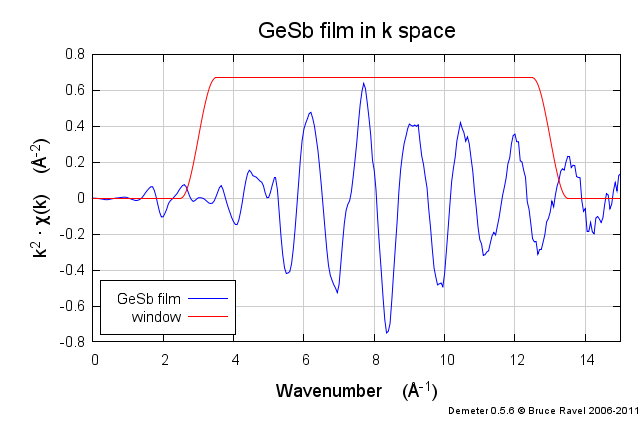
\includegraphics[width=0.8\linewidth]{../ATEA/info/gesb_chik.png}
      \end{center}
    \end{column}
    \begin{column}{0.5\linewidth}
      \begin{center}
        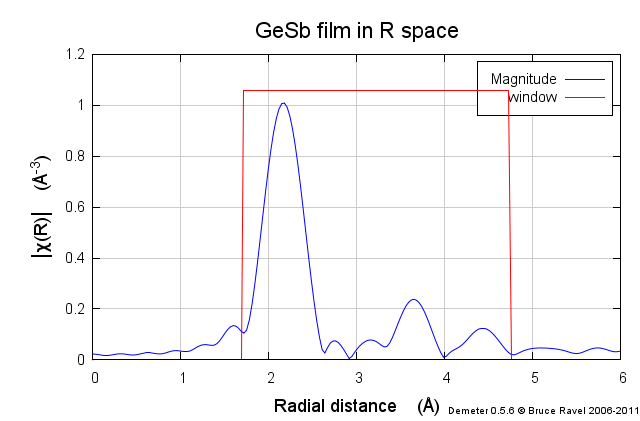
\includegraphics[width=0.8\linewidth]{../ATEA/info/gesb_chir.png}
      \end{center}
    \end{column}
  \end{columns}
  Here, I show a Fourier transform window of [3\,:\,13] and I suggest a
  fitting range of [1.7\,:\,4.7].  Applying the Nyquist criterion:
  \begin{equation}
    \notag N_{idp} \approx \frac{2\Delta k\Delta R}{\pi} \approx \alert{19}
  \end{equation}

  ~\\[-7ex]
  ~

  \begin{exampleblock}{}
    \begin{center}
      Did I really need to measure 5 scans?  Could I have stopped
      after a single scan?
    \end{center}
  \end{exampleblock}
  \begin{textblock*}{0.4\linewidth}(0pt,19.25\TPVertModule)%
    \tiny%
    These data are courtesy of Joseph Washington and Eric
    Joseph (IBM Research)
  \end{textblock*}
\end{frame}

\begin{frame}
  \frametitle{On all the rest of the days...}
  \small%
  ... we measure ... ummm ... less-than-beautiful data.  This is the
  merge of 42 scans on a solution containing 3\,mM of Hg bound to a
  synthetic DNA complex, measured in fluorescence at APS 20BM.
  \begin{columns}
    \begin{column}{0.5\linewidth}
      \begin{center}
        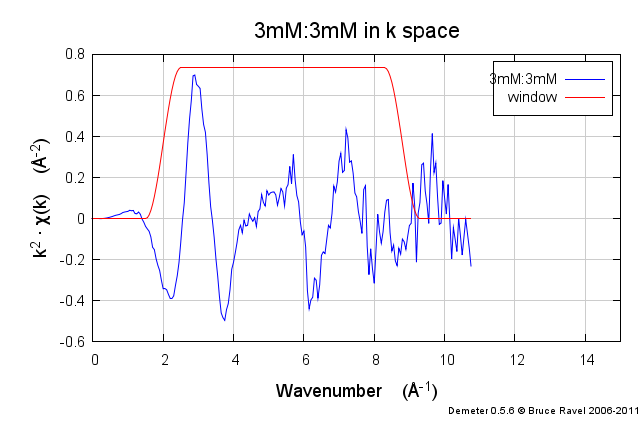
\includegraphics[width=0.8\linewidth]{../ATEA/info/hgdna_chik.png}
      \end{center}
    \end{column}
    \begin{column}{0.5\linewidth}
      \begin{center}
        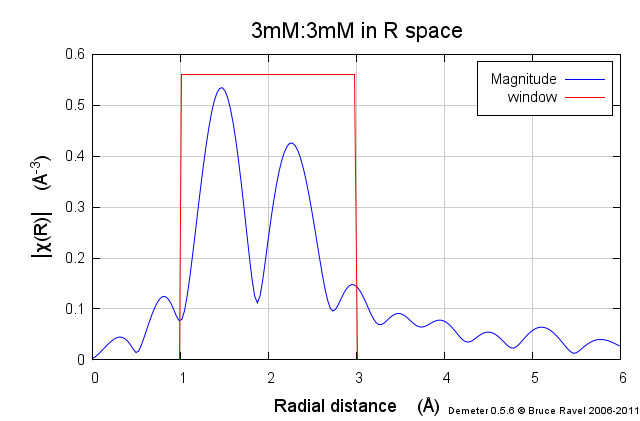
\includegraphics[width=0.8\linewidth]{../ATEA/info/hgdna_chir.png}
      \end{center}
    \end{column}
  \end{columns}
  Here, I show a Fourier transform window of [2\,:\,8.8] and I suggest a
  fitting range of [1\,:\,3].  Applying the Nyquist criterion:
  \begin{equation}
    \notag N_{idp} \approx \frac{2\Delta k\Delta R}{\pi} \approx \alert{8}
  \end{equation}

  ~\\[-7ex]
  ~

  \begin{exampleblock}{}
    \begin{center}
      Many real research problems are more like this.  Why were 42
      scans measured?  Was that too many?  Not enough?  How can we know?
    \end{center}
  \end{exampleblock}

  \begin{textblock*}{0.7\linewidth}(0pt,19.0\TPVertModule)%
    \tiny%
    B.\ Ravel, et al., \textit{EXAFS studies of catalytic DNA sensors
      for mercury contamination of water}, Radiation Physics and
    Chemistry \textbf{78}:10 (2009) pp\ S75-S79.
    \href{http://dx.doi.org/10.1016/j.radphyschem.2009.05.024}
    {\color{Blue4}\texttt{DOI:10.1016/j.radphyschem.2009.05.024}}
  \end{textblock*}
\end{frame}


\begin{frame}
  %\frametitle{The Central Limit Theorem}
  \begin{clt}
    Given certain conditions, the mean of a sufficiently large number
    of independent random variables, each with finite mean and
    variance, will be approximately normally distributed.
  \end{clt}

  \bigskip

  In the context of an EXAFS measurement, the CLT tells us that, when a
  noisy spectrum that is dominated by statistical noise, the spectral
  noise will be distributed normally about its mean.

  \bigskip

  If we measure enough repetitions of data dominated by statistical
  noise and merge the data by computing the arithmetic mean at every
  energy point, the data will converge to the mean.

  \begin{block}{In short...}
    With patience, ugly data becomes beautiful.
  \end{block}
\end{frame}


\section{Practical matters}

\begin{frame}
  \frametitle{The most basic rule of thumb}
  Before making a measurement, you have no idea what the data will
  look like.  You \textbf{cannot} know how many repetitions will be
  required before examining the first scan.
  \begin{description}
  \item[One scan?] Never$^*$ measure a single scan.  How would you
    know if something went wrong with the measurement?
  \item[Two scans?] What if the two repetitions are different?  How do
    know which one is right?
  \item[Three scans?] There you go!  Now you can know which on is
    right.  \alert{Always plan on at least three repetitions.}
  \end{description}
  \begin{textblock*}{0.7\linewidth}(0pt,17.5\TPVertModule)%
    \footnotesize%
    $^*$ Did I just say ``never''?  Yikes!  \textbf{Never} say
    ``never''!\\Why, on the very next page I am going to show examples
    where single scans were measured.
  \end{textblock*}
\end{frame}

\begin{frame}
  \frametitle{Rules of thumb always have exceptions...}
  \small
  \begin{columns}[T]
    \begin{column}{0.5\linewidth}
      Here are some time-resolved data.  Clearly we cannot take more
      than one scan under any set of conditions. Time marches on.        
    \end{column}
    \begin{column}{0.5\linewidth}
      These EXAFS data were taken at points in a rather large
      fluorescence imaging map.  To cover a large area, we only had time
      to measure a single scan per point.
    \end{column}
  \end{columns}

  \medskip

  \begin{columns}[T]
    \begin{column}{0.5\linewidth}
      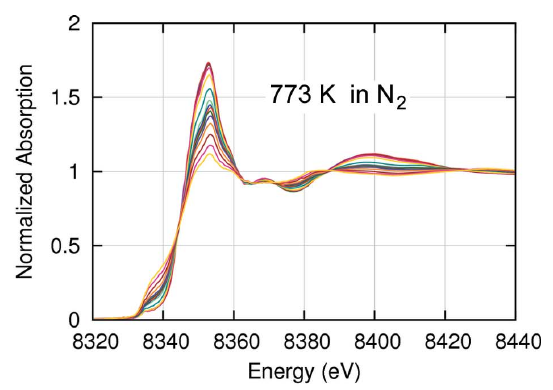
\includegraphics[width=\linewidth]{images/timeseq.png}
    \end{column}
    \begin{column}{0.5\linewidth}
      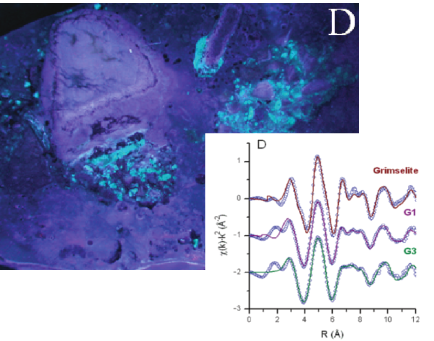
\includegraphics[width=\linewidth]{images/mapexafs.png}
    \end{column}
  \end{columns}
  \begin{textblock*}{0.4\linewidth}(0pt,18.0\TPVertModule)%
    \tiny%
    B.\ Ravel, et al., \textit{Simultaneous XAFS measurements of
      multiple samples}, J. Synchrotron Rad. (2010). \textbf{17}, pp\
    380-385 \href{http://dx.doi.org/10.1107/S0909049510006230}
    {\color{Blue4}\texttt{DOI:10.1107/S0909049510006230}}
  \end{textblock*}
  \begin{textblock*}{0.4\linewidth}(11\TPHorizModule,18.0\TPVertModule)%
    \tiny%
    D.H.\ Phillips, et al., \textit{Deposition of Uranium Precipitates
      in Dolomitic Gravel Fill}, Environ. Sci. Technol. (2008)
    \textbf{42}:19, pp\ 7104–7110
    \href{http://dx.doi.org/10.1021/es8001579}
    {\color{Blue4}\texttt{DOI:10.1016/10.1021/es8001579}}
  \end{textblock*}
\end{frame}

\begin{frame}
  \frametitle{When are data dominated by statistical noise?}
  \begin{block}{}
    Any of the following issues will contribute systematic uncertainty
    to you data.  If any of these are large compared to shot noise,
    then the CLT will not be observed in a data ensemble.
  \end{block}
  \begin{enumerate}
  \item Your sample is well made
    \begin{itemize}
    \item homogeneous in the distribution of the absorber
    \item of an appropriate thickness
    \item no Bragg diffraction from the sample or the matrix
    \end{itemize}
  \item Your detectors are linear
    \begin{itemize}
    \item well constructed
    \item not saturated
    \item the entire signal chain is in a linear regime
    \item no induced noise on the signal chain
    \end{itemize}
  \item The source and all optics are stable in temperature and
    vibration
  \item Harmonic content is eliminated from the beam
  \item The beam strikes the sample and only the sample
  \end{enumerate}
  \begin{alertblock}{}
    If all of those conditions are met, the variance in your data will
    be statistical and subject to the CLT.
  \end{alertblock}
\end{frame}

\begin{frame}
  \frametitle{Making decisions with real data}
  \begin{center}
    Here is some pretty noisy data of Co on carbon:

    \bigskip

    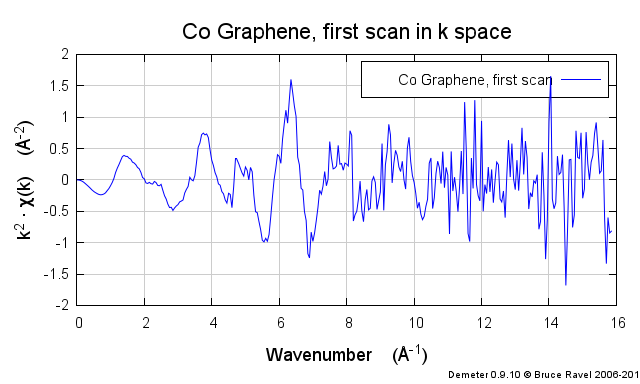
\includegraphics[width=0.7\linewidth]{images/firstscan.png}

    \bigskip

    Three repetitions will not be enough.
  \end{center}
\end{frame}

\section{Statistical analysis}

\begin{frame}
  \frametitle{An ensemble of data}
  \begin{columns}[T]
    \begin{column}{0.5\linewidth}
      \centering Here, again, is our one noisy scan\\[2.5ex]
      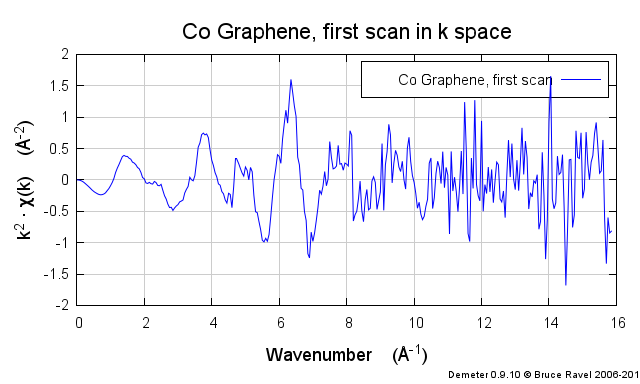
\includegraphics[width=\linewidth]{images/firstscan.png}
    \end{column}
    \begin{column}{0.5\linewidth}
      \centering ... and here are 45 scans I measured on a weekend day\\
      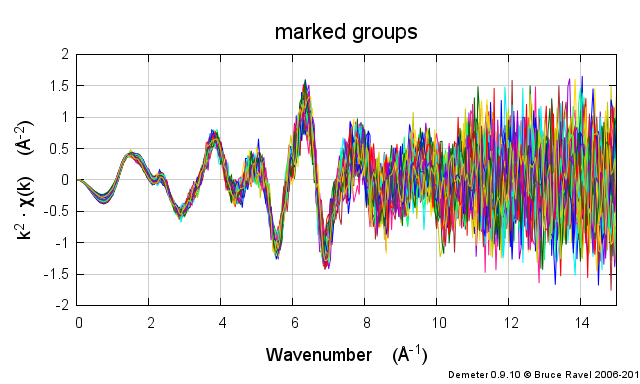
\includegraphics[width=\linewidth]{images/manyscans.png}
    \end{column}
  \end{columns}
  \begin{block}{}
    \centering Do these converge to the mean?
  \end{block}
\end{frame}

\begin{frame}
  \frametitle{The data merged}
  \begin{columns}[T]
    \begin{column}{0.5\linewidth}
      Here is the single scan compared as $k^2\cdot\chi(k)$ to the merge of all 45
      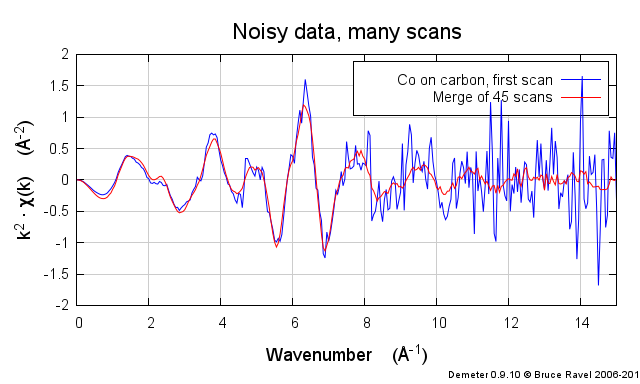
\includegraphics[width=\linewidth]{images/merge_chik.png}
    \end{column}
    \begin{column}{0.5\linewidth}
      \centering And as $|\tilde\chi(R)|$\\[2.5ex]
      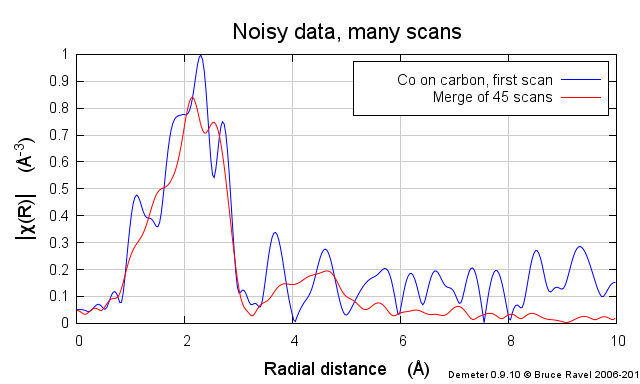
\includegraphics[width=\linewidth]{images/merge_chir.png}
    \end{column}
  \end{columns}
  \begin{block}{}
    A day's worth of patience paid off!  The merge of the 45 scans is
    fairly beautiful data, even if each individual scan seems
    hopelessly noisy.
  \end{block}
\end{frame}

\begin{frame}
  \frametitle{Convergence to the mean}
  \begin{columns}
    \begin{column}{0.5\linewidth}
      Here are successive samplings of this data ensemble showing the
      convergence to the mean. \\
      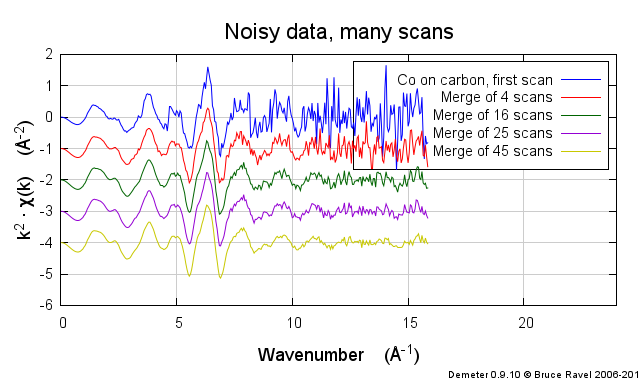
\includegraphics[width=\linewidth]{images/CoGr.png}
    \end{column}
    \begin{column}{0.5\linewidth}
      \small
      \begin{tabular}[h]{cccc}
        scans & $\sqrt{N}$ & $\epsilon_k$ & $\epsilon_1/\epsilon_N$ \\
        \hline\\
        1   & 1   & $3.147\times 10^{-3}$ & 1 \\
        4   & 2   & $1.686\times 10^{-3}$ & 1.9 \\
        16  & 4   & $7.719\times 10^{-4}$ & 4.1 \\
        25  & 5   & $6.307\times 10^{-4}$ & 5.0 \\
        45  & 6.7 & $3.974\times 10^{-4}$ & 8.0
      \end{tabular}
    \end{column}
  \end{columns}
  \begin{exampleblock}{}
    That worked well!  Apparently this sample was well-made and the
    beamline components were stable and linear.  The central limit
    theorem works!  Yay!
  \end{exampleblock}
\end{frame}


\begin{frame}
  \frametitle{Data limitations}
  Here are 142 repetitions of a measurement on Cr$_2$O$_3$.  These
  were measured at the same beamline and with the same detector as the
  previous data.  The merge changes little after 16 scans.

  \bigskip

  \begin{columns}[T]
    \begin{column}{0.5\linewidth}
      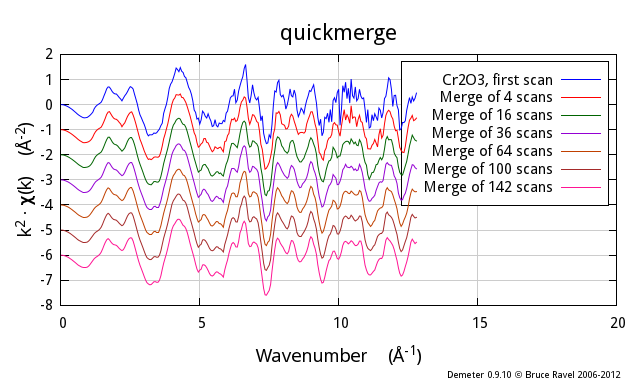
\includegraphics[width=\linewidth]{images/cr2o3.png}
    \end{column}
    \begin{column}{0.5\linewidth}
      \small
      \begin{tabular}[h]{cccc}
        scans & $\sqrt{N}$ & $\epsilon_k$ & $\epsilon_1/\epsilon_N$ \\
        \hline\\
        1   & 1  & $3.038\times 10^{-3}$ & 1 \\
        4   & 2  & $1.420\times 10^{-3}$ & 2.1 \\
        16  & 4  & $8.339\times 10^{-4}$ & 3.6 \\
        36  & 6  & $7.185\times 10^{-4}$ & 4.2 \\
        64  & 8  & $5.873\times 10^{-4}$ & 5.2 \\
        100 & 10 & $5.419\times 10^{-4}$ & 5.6 \\
        142 & 11.9 & $5.072\times 10^{-4}$ & 6.0
      \end{tabular}
    \end{column}
  \end{columns}

  \bigskip

  \begin{alertblock}{}
    \centering What's going on here?
  \end{alertblock}
\end{frame}

\begin{frame}
  \frametitle{Systematic uncertainty}

  \begin{block}{Statistical and systematic noise}
    More repetitions only solves the problem of statistical noise.
    There is systematic error -- probably sample inhomogeneity -- in
    these Cr$_2$O$_3$ data at the level of $\epsilon_k \approx 5\times
    10^{-4}$.
  \end{block}

  \bigskip

  Several things can cause systematic problems, including
  \begin{itemize}
  \item Monochromator glitches
  \item Sample inhomogeneity
  \item Non-linear detectors and/or signal chains
  \item Unstable mirrors or monochromator
  \item Gremlins!  (No food after midnight!)
  \end{itemize}
\end{frame}

\begin{frame}
  \frametitle{An example of a gross systematic problem}

  Here's an obvious example of a systematic problem.  These data were
  measured with a detector that has an energy-dependent non-linearity.

  \begin{columns}[T]
    \begin{column}{0.5\linewidth}
      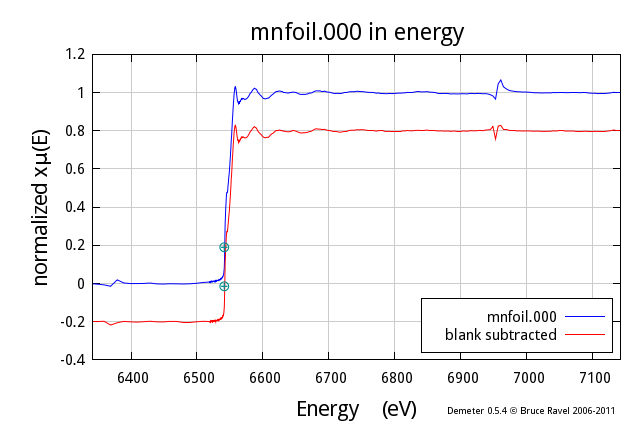
\includegraphics[width=\linewidth]{images/mnxmu.png}      
    \end{column}
    \begin{column}{0.5\linewidth}
      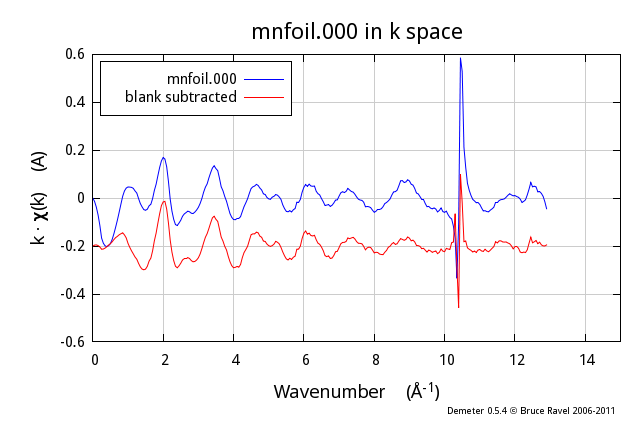
\includegraphics[width=\linewidth]{images/mnchik.png}      
    \end{column}
  \end{columns}

  \bigskip

  \begin{alertblock}{}
    No number of repetitions will ever fix that feature of the data.
    The \textbf{only} solution is to fix the detection problem.
  \end{alertblock}
\end{frame}

\section{Conclusions}

\begin{frame}
  \frametitle{Beating down noise can be a fool's game}
  \small%
  \begin{center}
    \alert{Counting statistics is mean-spirited and $N^2$ is an
      unhappy requirement.}
  \end{center}

  \begin{center}
    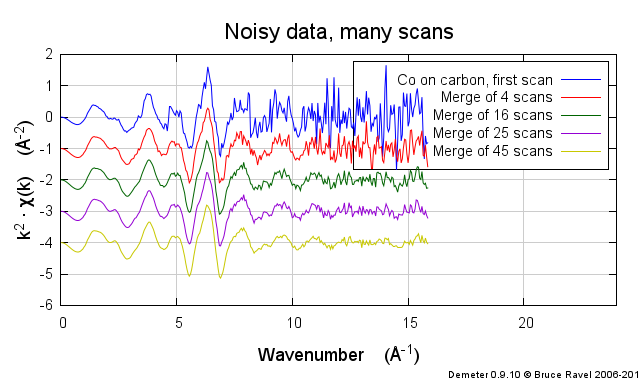
\includegraphics[width=0.55\linewidth]{images/CoGr.png}
  \end{center}

  Here again is the convergence of the Co on carbon data.
  It took 45 scans -- about 13 hours at my beamline -- to turn these
  data into the sort of excellent EXAFS data we like to work on.  We
  typically give users 3 days of beam time, enough for 5 or 6 such
  samples.

  \bigskip

  \begin{alertblock}{}
    Sometimes we have to compromise on data quality in order to
    measure enough samples to make a full experiment.
  \end{alertblock}
\end{frame}

\begin{frame}
  \frametitle{... but can really be worth it}

  \begin{exampleblock}{}
    The Central Limit Theorem always works!  If data is important
    enough to you, it can be measured.
  \end{exampleblock}

  \begin{center}
    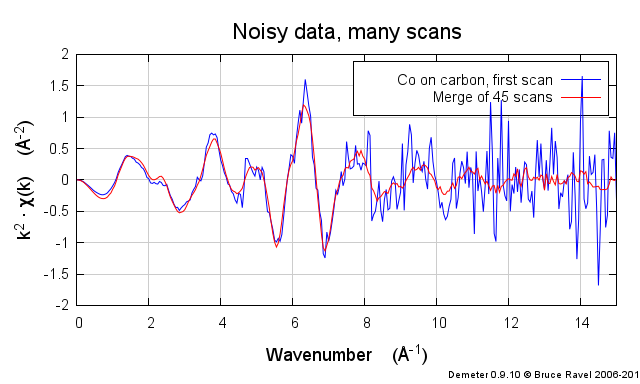
\includegraphics[width=0.55\linewidth]{images/merge_chik.png}

    \bigskip

    The collection of these data required only a simple calculation and
    a bit of patience.
  \end{center}
\end{frame}

\begin{frame}
  \frametitle{... except when it isn't!}
  \begin{alertblock}{}
    The Central Limit Theorem only works when your data are dominated
    by statistical noise.
  \end{alertblock}

  \begin{columns}[T]
    \begin{column}{0.5\linewidth}
      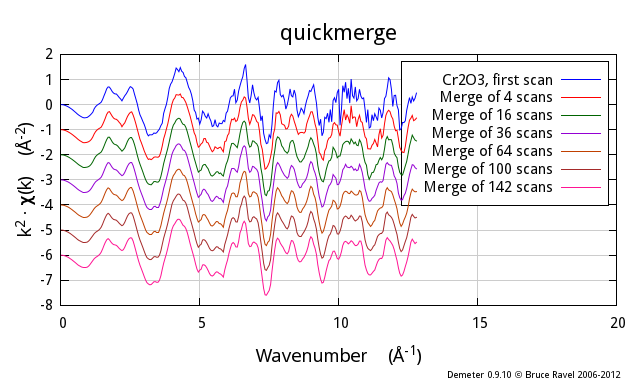
\includegraphics[width=\linewidth]{images/cr2o3.png}

      \bigskip

      The collection of scan 17 (or perhaps scan 5!) through scan 142
      was a poor use of time.
    \end{column}
    \begin{column}{0.5\linewidth}
      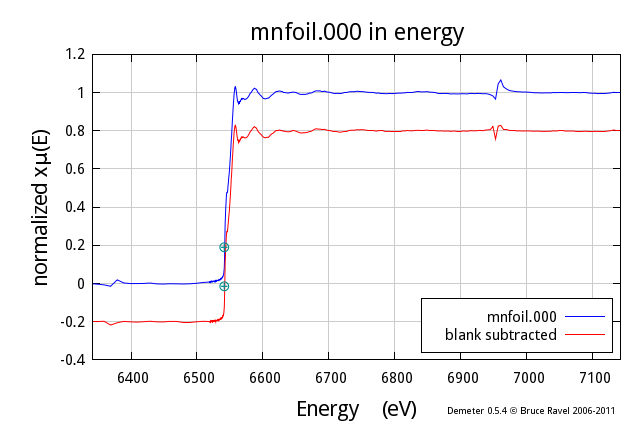
\includegraphics[width=\linewidth]{images/mnxmu.png}  

      \bigskip
    
      No amount of data repetition fixes a detector (or sample
      or mono or...) problem.
    \end{column}
  \end{columns}
\end{frame}

\begin{frame}
  \frametitle{Designing a real experiment (1)}
  \begin{block}{Here are the sorts of questions you need to ask
      yourself at the beginning of a new project}
    \begin{enumerate}
    \item How much beam time do you have?  How long does a scan
      typically take at the beamline you will be visiting?  How
      many samples do you have?
    \item Have you considered how best to prepare your sample?  Will
      you be measuring in transmission or fluorescence?
    \item Will XANES data suffice?  Or do you need high quality EXAFS
      data?
    \item Have you prioritized your samples in case collection of
      adequate data takes longer than you planned?
    \end{enumerate}
  \end{block}
\end{frame}

\begin{frame}
  \frametitle{Designing a real experiment (2)}
  \begin{exampleblock}{Here are the sorts of questions you need to ask
      yourself once you begin collecting data}
    \begin{enumerate}
    \item What does the first scan look like?
    \item Will XANES data suffice?  Or do you need high quality EXAFS
      data?
    \item On the basis of the noise, how many scans will be required
      for beautiful data?
    \item How many scans for usable data?
    \end{enumerate}
  \end{exampleblock}
\end{frame}

\end{document}



%%% Local Variables:
%%% TeX-parse-self: t
%%% TeX-auto-save: t
%%% TeX-auto-untabify: t
%%% TeX-PDF-mode: t
%%% End:
